\chapter{Formáty využívající se v API}
V této kapitole budou popsány především dva základní formáty dat které jsou stále aktivní -- JSON a XML.


\subsection*{Serializace a deserializace} %TODO cote https://www.baeldung.com/cs/serialization-deserialization
Serializace a deserializace jsou důležité koncepty v programování. Umožňují ukládat, přenášet a znovu sestavit data. Používají se celou řadu věcí, jako je ukládání objektů do databáze, posílání dat po síti a nebo pro účely mezipaměťi.

Objekt má 3 základní vlastnosti: identitu, stav a chování. Stav reprezentuje jednotlivá data objektu.
\textbf{Serializace} je proces převádění stavu objektů do proudu bytů co mohou být kdekoliv uloženy nebo poslány. Tento proud může být poté zase rekonstruován do původního objektu. Pro serializaci si však muíme vybrat formát dat. Jako třeba JSON nebo XML. Ovšem používá se i binární reprezentace dat. Tato reprezentace se často využívá pro výkonnostní potřeby, protože jsou typicky rychlejší na zápis a čtení. Jejich nevýhoda ale je, že nejsou člověkem čitelné.

\textbf{Deserializace} je opačný proces od serializace. Tedy převedení proudu bytů zpátky do objektu.

Jednou z nevýhod serializace a deserializace jsou vysoké nároky na výkon. Můžeto trvat nezanedbatelné množství času. Zvlášť u velkých objektů. Za zmínku stojí i fakt, že ne všechny objekty mohou být serializovány. Jako třeba sockety nebo file handlery.


\section{JSON}
JavaScript Object Notation neboli JSON je formát, který je odvozen z Javascriptu, nicméně mnoho dnešních jazyků už má serializaci do JSONu zabudovanou interně. Jedná se o textový formát zápisu objektů, který je dobře čitelný člověkem. Ukládá data do párů \textbf{key:value} kdy key je klíč a value hodnota, která je pod ním uložená, obvykle může jít o číslo, textový řetězec, pole nebo i další objekt. Znaky v JSONu musí být v kódování UTF-8, ale formát podporuje i speciální znaky pokud jsou escaped, jako příklad můžeme uvést znaky \verb |\uD83D\uDE10| nebo \textit{neutral-face}. JSON je využíván primárně k výměně dat mezi webovými aplikacemi a servery, ale dá se používat i pro jednoduché databáze. Má prostá ale zato striktní pravidla a tudíž je jednoduché zkontrolovat jeho správnost. Jeden z jeho nedostatků je, že nemá podporu komentářů oproti XML, které tuto podporu má. %\textbf{ TODO odkaz někde na iso normu https://www.iso.org/standard/71616.html} %TODO bibtech na iso normu plus dát emoji 😐 třeba xetex ale to se pak celé rozbije


\subsection{Pravidla}
\textbf{Key} neboli klíč daného objektu je vždy string a reprezentuje název určitého atributu. \textbf{Value} představuje hodnotu, kterou tento atribut nabývá a může být datového typu text, číslo, logická hodnota, null, další objekt či pole. Jednotlivé atributy jsou vždy odděleny čárkou. Jako příklad je uveden JSON objekt z API modelové hry, který popisuje hráče, jeho vlastnosti a jeho rasu, reprezentovanou jako vnořený objekt.

\begin{listing}[H]
  \inputminted{json}{resources/code/standards/player.json}
  \caption{Příklad JSON objektu}
  \label{code:json_player}
\end{listing}

V tomto JSONu můžeme vidět všechno, s čím se u tohoto datového formátu můžeme setkat. Jako první atribut, tento objekt má \verb|"id":4|, kde id je klíč a 4 je číslo -- to značí, že tento objekt má svůj unikátní identifikátor 4.

Na 6 řádku můžeme vidět atribut \verb|"title":"Elf"|. Value je v tomto případě text, který poznáme podle zaobalení uvozovek. Tento řádek v kontextu celého objektu značí, že se jedná o rasu postavy, která má název \textit{Elf}.

Atribut, který tento text zaobaluje, je \texttt{"race"}. Jedná se o příklad objektu, v tomto případě rasy, která má své vlastnosti reprezentované právě tímto objektem.

V atributu \texttt{"effects"} se nachází pole objektů. V tomto případě to jsou objekty obsahující klíč s id rasy a jejím efektem, ke kterému je přidána také informace o tom, od jaké úrovně je tento efekt zpřístupněn. Podobně tak na řádku 26 je jako value klíče \texttt{inventory} pole textových řetězců znázorňující předměty, které hráč vlastní.

Dále si můžeme povšimnout atributu \texttt{clazz} na řádku 3, který má hodnotu \texttt{null}. To nám značí, že tento konkrétní klíč u objektu zatím nic neobsahuje. Může se stát že jen nebyl přiřazen a v budoucnu nějakou hodnotu dostane.

A nakonec zde máme na řádku 29 atribut \texttt{dead} s hodnotou \texttt{false}. Tato hodnota značí logickou hodnotu, která má datový typ boolean. V našem případě se jedná o vlastnost, která nám říká, zda je hráč mrtvý (\texttt{true}) či nikoli (\texttt{false}).


\section{XML}
Extensible Markup Language je jazyk primárně určený na serializaci a přenášení dat, který je podobně jako JSON čitelný i člověkem. Základní stavební blok je node, atributy jsou uloženy do párů kterým říkáme tagy. Za pomocí své deklarace podporuje určení kódování a různé verze. Díky XML Schema definition také podporuje celou řadu datových typů a oproti JSONu podporuje i komentáře. Standardy spravuje společnost W3C. %\textbf{fest fajny odkaz na w3c specifikaci do bibtex} %TODO bibtech na w3c


\subsection{Pravidla}
Na začátku dokumentu je vždycky XML deklarace, která určuje, o jakou verzi se jedná a jaké mají znaky kódování.
Samotná data jsou zaznamenána pomocí párových tagů, dohromady nazývaným \textbf{element}, které se zapisují jako počáteční (\texttt{<character>}) a ukončovací (\texttt{</character>}) tag, kde \textit{character} značí název atributu, podobně jako \textbf{key} u JSONu. Hodnota atributu se píše buď mezi počáteční a ukončovací tag, nebo přímo do tagu samotného (\texttt{<character id=4>}). Tzv. \textit{procesory} analyzují XML dokumenty a posílají dále strukturovaná data aplikaci, která se využívá. Procesory můžou být jak validující tak nevalidující, přičemž validující musí nalezenou chybu nahlásit ale pořád mohou v parsování pokračovat.

\begin{listing}[H]
  \inputminted{xml}{resources/code/standards/player.xml}
  \caption{Příklad XML dokumentu i se schématem}
  \label{code:xml_player}
\end{listing}

\begin{figure}[H]
  \centering
  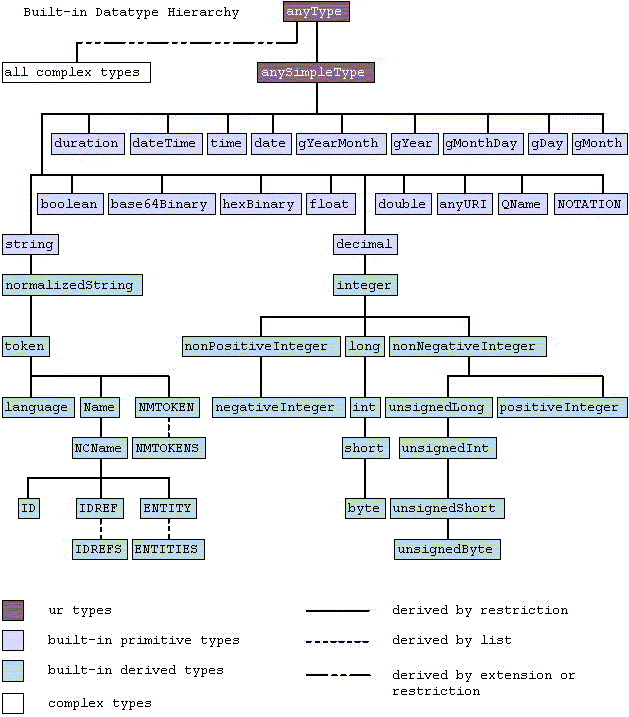
\includegraphics[width=0.7\textwidth]{figures/type-hierarchy.png}
  \caption{Hierarchie datových typů v XML schema}%\cite{british_museum_2021}}
  \label{fig:xml_datatypes}
\end{figure}
%TODO odkaz na obrázek všech možných datových typů https://www.w3.org/TR/xmlschema-2/type-hierarchy.gif a přímo ta stránka https://www.w3.org/TR/xmlschema-2/#built-in-datatypes


%TODO nějaký odkaz pěkný nebo tak něco na 
Tento XML dokument reprezentuje stejnou strukturu jako JSON popsaný výše. Oproti němu je však rozšířen o schéma, ve kterém můžeme určit jeden z mnoha datových typů \ref{fig:xml_datatypes} pro každý element (řádek 3) či atribut (řádek 6 a 7). Když není schéma specifikováno, všechny datové typy jou brány za text. Velká změna oproti JSONu také spočívá v tom, že víme, o jaký objekt se jedná (řádek 23 a 48) -- místo obyčejných složených závorek zde máme element se jménem \textit{character}, což je informace, kterou JSON neposkytuje.


\section{Shrnutí}
Teď byly představeny případné technologie co bychom mohli použít jako formát pro serializaci a deserializaci. Jak tyto technologie fungují, jak vypadají a jejich výhody a nevýhody.

\begin{table}[h]
  \centering
  \begin{tabular}{|l|c|c|c|c|}
    \hline
           & Čitelnost & Jednoduchost & Rychlost & Skladnost \\
    \hline
    JSON   & 1         & 1            & 2        & 3         \\
    \hline
    XML    & 2         & 3            & 4        & 4         \\
    \hline
    Binary & 5         & 4            & 1        & 1         \\
    \hline
  \end{tabular}
  \caption{Porovnání JSON, XML a Binary }
  \label{tab:formats_comparison}
\end{table}

\tableref{tab:formats_comparison} nám srovnává různé technologie podle našich případných požadavků. \footnote[1]{Známkování jsem prováděl čistě podle vlastního uvážení co bude pro naše použití nejvhodnější} \footnote[2]{Známkování je od 1 do 5 kdy 1 představuje souhlas a 5 nesouhlas} Pro naše účely je potřeba něco jednoduchého a srozumitelného, přiměřeně rychlého. Tedy nejlépe z toho vyplývá JSON. XML je pro naše účely moc komplexní a většinu vlastností nevyužijeme. Binární formát je sice rychlý ale špatně se odhalují chyby a je zde horší universálnost serializeru a deserializeru mezi jazyky.


\endinput